\begin{enumerate}[label=\thesubsection.\arabic*.,ref=\thesubsection.\theenumi]
\numberwithin{equation}{enumi}

\item Consider the circuit given below, here $R_1$= 1K$\Omega$ , $R_2$= 2K$\Omega$ , $C_1$= $C_2$= 1\emph{mF}.Both the capacitors were charged to 1 C. Find Differential equations for $q_1$ and $q_2$.


\begin{figure}[!ht]
    \begin{center}
		
		\resizebox{\columnwidth}{!}{\begin{circuitikz}[american, scale = 1.5][americanvoltages]
      \draw (0,0)
      to[short] (0,2) % The voltage source
      to[short] (2,2)
      to[R =$R_1$, i=$i_1$] (2,1) % The resistor
      to[C,v^<=$C_1$] (2,0) % Capacitor One
      to[short] (0,0);
      \draw (2,2)
      to[short] (4,2)
      to[R=$R_2$, i=$i_2$] (4,1)
      to[C,v^<=$C_2$] (4,0)
      to[short] (2,0);
      \draw (0,0) to[short] node[ground] {} (0,-0.1);
\end{circuitikz}
}
	\end{center}
\caption{Circuit diagram}
\label{fig:circuit_diagram}
\end{figure}

\solution We know that, $i_1$ = -$\dot{q_1}$ , $i_2$ = -$\dot{q_2}$   ('-' as charge is depleting)\\
Applying \emph{KVL} on 1st branch we get:
\begin{align}
    -\dot{q_1}R_1 - \frac{q_1}{c_1} = 0\\
    \dot{q_1} = -q_1
\end{align}
Now, Applying \emph{KVL} 0n 2nd branch we get:
\begin{align}
    -\dot{q_2}R_2 - \frac{q_2}{c_2} = 0\\
    \dot{q_2} = -2q_2
\end{align}

If I represent this as state space model\\
Taking $x = \myvec{q_1\\q_2}$\\
And here $x(0) = \myvec{q_1(0)\\q_2(0)} = \myvec{1\\1}$\\
$\therefore$ State space model can be represented as \\
\begin{align}
    \dot{x} = \myvec{-q_1 \\ -2q_2} = \myvec{-1 & 0\\0 & -2}x
\end{align}
\newline


\item  Consider the linear system :
\begin{align}
    \dot{x} = \myvec{-1 & 0\\0 & -2}x
\end{align}
with initial condition:  
x(0) = \myvec{1\\1}. Find x(t)


(A) x(t) =
\myvec{
e^{-t} & te^{-2t}\\
0 & e^{-2t}
}
\myvec{
1\\
1
}

\\

(B) x(t) =
\myvec{
e^{-t} & 0\\
0 & e^{2t}
}
\myvec{
1\\
1
}

\\

(C) x(t) =
\myvec{
e^{-t} & t^{2}e^{-2t}\\
0 & e^{-2t}
}
\myvec{
1\\
1
}

\\

(D) x(t) =
\myvec{
e^{-t} & 0\\
0 & e^{-2t}
}
\myvec{
1\\
1
}\\
\\
\solution Given expression is the state equation, as it can be written in the following form
\begin{align}
    \dot{x} =Ax + BU
\end{align} \\
Here, A =  \myvec{-1 & 0\\0 & -2} and U = 0\\
Solution to this can be given by
\begin{align}
    x(t) = \phi(t)x(0)
\end{align}
Where $\phi(t)$ is called the state-transition matrix and is given by\\
\begin{align}
    \phi(t) = \mathscr{L}^{-1}\myvec{\myvec{sI -A}^{-1}}
\end{align}\\
\begin{align}
    \myvec{sI-A} = \myvec{s+1 & 0\\ 0 & s+2}
\end{align}\\
\begin{align}
    \myvec{sI-A}^{-1} 
    = \myvec{\frac{1}{s+1} & 0\\
            0 & \frac{1}{s+2}}
\end{align}
\begin{align}
    \mathscr{L}^{-1}\myvec{\myvec{sI -A}^{-1}} = \myvec{
e^{-t} & 0\\
0 & e^{-2t}
}
\end{align}
Given x(0) = \myvec{1 \\ 1}
\begin{align}
    \therefore x(t) = \myvec{
e^{-t} & 0\\
0 & e^{-2t}
}
\myvec{
1\\
1
}\\ 
\therefore option (D)   
\end{align}
\newline
\newline

\emph{*Derivation for state transition matrix:}
\begin{align}
    \dot{x} =Ax
\end{align} 
Applying laplace transform, we get
\begin{align}
    sX(s) -x(0) = AX(s)\\
    \myvec{sI - A}X(s) = x(0)\\
    X(s) = \myvec{sI - A}^{-1}x(0)\\
\end{align} 
Taking inverse laplace transform
\begin{align}
    x(t) = \mathscr{L}^{-1}\myvec{\myvec{sI -A}^{-1}}x(0)
\end{align}
$\to$ Where $\mathscr{L}^{-1}$\myvec{\myvec{sI -A}^{-1}} is called State transition matrix.\\
\item Draw block diagram for the the above mentioned state model.\\
\solution Here, clearly Transfer function is given by 
\begin{align}
    X(s) = \myvec{sI - A}^{-1}x(0)
\end{align}
Input being constant = x(0), and output is X(s)\\
\begin{align}
    X_1(s) = \frac{1}{s+1}x_1(0)\\
    X_2(s) = \frac{1}{s+2}x_2(0)
\end{align}
Lets consider a closed loop negative unity feed back system, We know its open loop gain
\begin{align}
    = \frac{G(s)}{1+G(s)}
\end{align}
We can re-write the above to transfer equations as
\begin{align}
    X_1(s) = \frac{\frac{1}{s}}{\frac{1}{s}+1}x_1(0)\\
    X_2(s) = \frac{\frac{1}{s+1}}{\frac{1}{s+1}+1}x_2(0)
\end{align}
Below are the block the block diagrams for $X_1$(s) and $X_2$(s)
\begin{figure}[!ht]
    \begin{center}
		
		\resizebox{\columnwidth}{!}{\tikzset{
        block/.style = {draw, rectangle,
            minimum height=1cm,
            minimum width=2cm},
        input/.style = {coordinate,node distance=1cm},
        output/.style = {coordinate,node distance=4cm},
        arrow/.style={draw, -latex,node distance=2cm},
        pinstyle/.style = {pin edge={latex-, black,node distance=2cm}},
        sum/.style = {draw, circle, node distance=1cm},
}

\begin{tikzpicture}[node distance=2.5cm,auto,>=latex']
  \node [input, name=input] {};
  \node [sum, right of=input] (sum) {};
  \node [block, right of = sum] (block1) {$\frac{1}{s}$};
  \node [output, right of= block1] (output) {};
  \draw [->] (input) -- node {$x_1(0)$} (sum);
  \draw [->] (sum) -- node {} (block1);
  \draw [->] (block1) -- node [name =y] {$X_1(s)$} (output);
  \draw [->] (y) -- ++ (0,-2) -| node [pos=0.99] {$-$} (sum);
\end{tikzpicture}
}
	\end{center}
\caption{block diagram for $X_1$}
\label{fig:block1}
\end{figure}
\begin{figure}[!ht]
    \begin{center}
		
		\resizebox{\columnwidth}{!}{\tikzset{
        block/.style = {draw, rectangle,
            minimum height=1cm,
            minimum width=2cm},
        input/.style = {coordinate,node distance=1cm},
        output/.style = {coordinate,node distance=4cm},
        arrow/.style={draw, -latex,node distance=2cm},
        pinstyle/.style = {pin edge={latex-, black,node distance=2cm}},
        sum/.style = {draw, circle, node distance=1cm},
}

\begin{tikzpicture}[node distance=2.5cm,auto,>=latex']
  \node [input, name=input] {};
  \node [sum, right of=input] (sum) {};
  \node [block, right of = sum] (block1) {$\frac{1}{s+1}$};
  \node [output, right of= block1] (output) {};
  \draw [->] (input) -- node {$x_2(0)$} (sum);
  \draw [->] (sum) -- node {} (block1);
  \draw [->] (block1) -- node [name =y] {$X_2(s)$} (output);
  \draw [->] (y) -- ++ (0,-2) -| node [pos=0.99] {$-$} (sum);
\end{tikzpicture}
}
	\end{center}
\caption{block diagram for $X_2$}
\label{fig:block2}
\end{figure}
\\
\item Describe how an oscillator works \\
\solution Oscillators convert a DC input (the supply voltage) into an AC output (the waveform) \\
\begin{figure}[!ht]
    \begin{center}
		
		\resizebox{\columnwidth}{!}{\tikzset{
        amp/.style = {regular polygon, regular polygon sides=3,
              draw, fill=white, text width=1em,
              inner sep=1mm, outer sep=0mm,
              shape border rotate=-90},
        block/.style = {draw, rectangle,
            minimum height=1cm,
            minimum width=2cm},
        input/.style = {coordinate,node distance=1cm},
        output/.style = {coordinate,node distance=4cm},
        arrow/.style={draw, -latex,node distance=2cm},
        pinstyle/.style = {pin edge={latex-, black,node distance=2cm}},
        sum/.style = {draw, circle, node distance=1cm},
}

\begin{tikzpicture}[node distance=2.5cm,auto,>=latex']
  \node [input, name=input] {};
  \node [sum, right of=input] (sum) {};
  \node [amp, right of = sum] (block1) {$A$};
  \node [output, right of= block1] (output) {};
  \node [block, below of = block1] (block2) {$B$};
  \draw [->] (input) -- node {$V_{in}$} (sum);
  \draw [->] (sum) -- node {$V_{in} + BV_{out}$} (block1);
  \draw [->] (block1) -- node [name =y] {$V_{out}$} (output);
  \draw [->] (y) |- node [above,pos=0.79] {$V_{out}$} (block2) ;
  \draw [->] (block2) -| node  {$BV_{out}$} (sum) ;
\end{tikzpicture}
}
	\end{center}
\caption{block diagram for oscillator}
\label{fig:block2}
\end{figure}
Given Below is basic block diagram\\
Resonant frequency, is the frequency at which oscillator oscillates, it depends on R/L/C components of the circuit it's been fed back through.\\
Oscillators work because they overcome the losses of their positive feedback circuit either in the form of a capacitor, inductor or both. In other words, an oscillator is a an amplifier which uses positive feedback that generates an output frequency without the use of an input signal.\\
Oscillators gain can be given as follows:\\
From the above circuit we have :\\
A = Amplifiers gain, B = positive feedback gain, G = total gain of the circuit
\begin{align}
    A(V_i_n + BV_o_u_t) =V_o_u_t \\
    G = \frac{V_o_u_t}{V_i_n} = \frac{A}{1 - AB}
\end{align}
We get,\\
sustained oscillations when $AB = 1$\\
Exponentially decaying oscillation for $AB<1$ \\
Exponentially increasing oscillation for $AB >1$ (unstable)\\
\newline
\item Hartley oscillator:\\
The Hartley oscillator is one of the classical LC feedback circuits,i.e feedback is made of LC components.Below here we can see a general form of any LC-type oscillator:

\begin{figure}[!ht]
    \begin{center}
		
		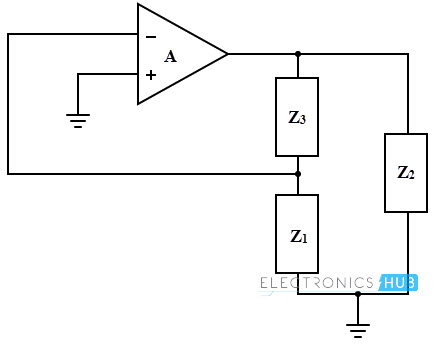
\includegraphics[scale=0.8]{./figs/blc.jpg}
	\end{center}
\caption{block diagram for oscillator}
\label{fig:block2}
\end{figure}

For any LC oscillator, 
\begin{align}
    Z_1 = jX_1\\
    Z_2 = jX_2\\
    Z_3 = jX_3\\
\end{align}
We know that feedback gain is B, i.e, $\frac{V_0}{V_f} = B$\\
Applyting voltage divider rule we get
\begin{align}
    B = \frac{Z_1}{Z_1 + Z_3}
\end{align}
Consider the below circuit
\begin{figure}[!ht]
    \begin{center}
		
		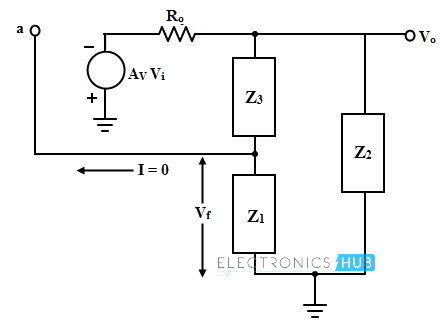
\includegraphics[scale=0.8]{./figs/lc.jpg}
	\end{center}
\caption{block diagram for oscillator}
\label{fig:block2}
\end{figure}
\begin{align}
    A = \frac{V_o}{V_{in}} = \frac{AZ_L}{R_o + Z_L}\\
    where\\
    Z_L = \frac{(Z_2 + Z_3)Z_1}{Z_1+Z_2+Z_3}\\
\end{align}
Now,we know that $AB = 1$ for sustained oscillations, putting the the above terms in the equation

    on solving,\\
\begin{align}    
    AB = \frac{Z_1Z_2A}{(Z_1+Z_2+Z_3)A+ Z_1(Z_2+Z_3)}\\
    Z_1 = jX_1,
    Z_2 = jX_2,
    Z_3 = jX_3\\
\end{align}    

    putting that in we get\\
\begin{align}
AB = \frac{AX_1X_2}{X_1(X_2+X_3) -jR_o(X_1+X_2+X_3)}
\end{align}
For hartley oscillator, 
\begin{align}
    Z_1 = j\omega L_1 (inductor)\\
    Z_2 = j\omega L_2 (inductor)\\
    Z_3 = \frac{1}{j\omega C} (capacitor)\\
\end{align}
Since, AB is real
\begin{align}
    X_1+X_2+X_3 = 0\\
\end{align}

    For, Hartley oscillator, substituting terms in above equation\\
\begin{align}    
    \omega L_1 + \omega L_2  = \frac{1}{\omega C}\\
    \omega = \frac{1}{\sqrt{(L_1+L_2)(C)}}\\
    f = \frac{1}{2\pi \sqrt{(L_1+L_2)(C)}}
\end{align}
\begin{align}
    B = \frac{Z_1}{Z_1 + Z_3} = \frac{Z_1}{Z_2}\\
      = \frac{L_1}{L_2}\\
    A =  \frac{L_2}{L_1} 
\end{align}
Given below is circuit for Hartley oscillator built using opamp\\
\begin{figure}[ht]
    \begin{center}
	    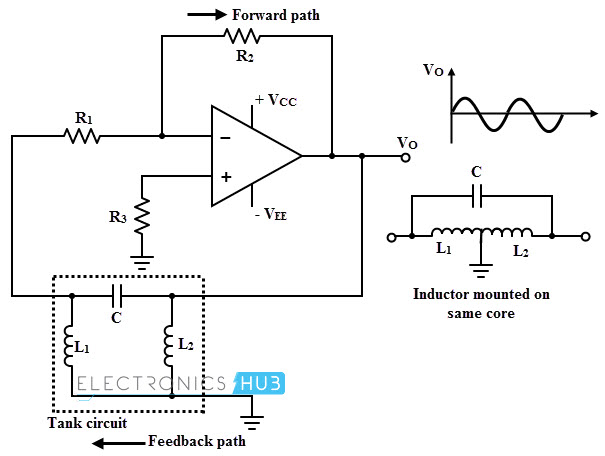
\includegraphics[scale=0.7]{./figs/hart.jpg}
	\end{center}
\caption{block diagram for oscillator}
\label{fig:block2}
\end{figure}
\item For Hartley oscillator frequency generated can be given as 
\begin{align}
    f = \frac{1}{2\pi\sqrt{(L_1 + L_2)C}}
\end{align}
Taking,
\begin{align}
   L_1 = 1 \mu H\\
   L_2 = 1 \mu H\\
   C = 1.2 pF
\end{align}
We get f = 103 MHz\\
Feedback factor for Hartley given by:
\begin{align}
Feedback factor =\frac{L_2}{L_1}= 1
\end{align}
W.K.T, $AB = 1$\\
$\therefore$ Minimum amplification Gain = 1
\end{enumerate}
